% Conclusion

\begin{frame}[c]
  \frametitle{Conclusion générale}

Les Frappes de Processus standard permettent une \tval{représentation atomique}\\
des réseaux de régulation biologique :
\begin{itemize}
  \item Analyse statique efficace existante
  \item Mais problèmes de décalage temporel
  \item Limites de modélisation
\end{itemize}

\medskip
\tval{Extensions des Frappes de Processus} pour augmenter l'expressivité :
\begin{itemize}
  \item Correction du décalage temporel \f expressivité strictement plus forte
  \item Possibilité de simuler des paramètres temporels
  \item Nouveaux liens avec d'autres formalismes (Thomas, RdP, etc.)
\end{itemize}

\medskip
Élargissement de l'\tval{analyse statique} à la forme canonique :
\begin{itemize}
  \item Analyse efficace de propriétés dynamiques
  \item Applicable aux différentes extensions au prix d'une traduction
  \item Nouveau type de propriétés : activation simultanée
\end{itemize}

% 
% 
% Process Hitting: an atomistic modeling with powerful static analysis
% 
% \medskip
% \begin{enumerate}[1.]
%   \item Stochastic parameters:
%     \begin{itemize}
%       \item To model systems with chronometric features
%       \item \tval{Continuous time}
%       \item But \tval{hard to analyze}
%     \end{itemize}
%   \item Classes of priorities:
%     \begin{itemize}
%       \item Allows to reproduce the same behaviors
%       \item Efficient \tval{static analysis}
%       \item But the translation to canonical form faces \tval{combinatorial explosion}
%     \end{itemize}
%   \item Neutralizing edges:
%     \begin{itemize}
%       \item Alternative to priorities
%       \item Closer to reality in some cases
%       \item \tval{Lighter translation} to canonical form
%     \end{itemize}
% \end{enumerate}
% 
% \vfill
% \Large
% \begin{flushright}
%   \tval{Thank you}\hspace{1cm}~
% \end{flushright}
% \vfill

\end{frame}

\setbeamercovered{invisible}



\begin{frame}[c]
  \frametitle{Ouvertures et perspectives}

Pistes d'\tval{exploitation} :
\begin{itemize}
  \item Modélisation et analyse de bases de données complètes
  \item Étude de comportements incontrôlables, de perturbations ponctuelles
  \item Recherche de propriétés intéressantes (attracteurs, oscillations...)
\end{itemize}

\medskip
Enrichissement de l'\tval{analyse statique} :
\begin{itemize}
  \item Raffinement pour réduire l'ensemble des cas non-conclusifs
  \item Utilisation de méthodes dérivées utilisant le graphe de causalité locale
  \item Développement de nouvelles propriétés (logiques temporelles, compteurs...)
\end{itemize}

\medskip
Enrichissement des \tval{capacités de représentation} :
\begin{itemize}
  \item Classes de priorités dynamiques
  \item Actions gardées ou portes logiques complexes
  \item Outils de vérification et correction (logique de Hoare)
\end{itemize}

\end{frame}



\begin{frame}[c]
  \frametitle{Collaborations}

Participation au projet \tval{ANR blanc BioTempo} (mars 2011 -- novembre 2014) :
\begin{center}
«~Représentations à l’aide de langage, de temps et de modèles hybrides\\
pour l’analyse de modèles incomplets en biologie moléculaire~»
\end{center}
Tâche 3 : Introduction de synchronisations\\
et de données chronométriques dans les modèles chronologiques

\bigskip
\bigskip
Stage doctoral de 3 mois (mars -- mai 2012) :\\
\tval{National Institute of Informatics} (Tokyo, Japon)\\
Invité dans l'équipe de \tval{Katsumi Inoue}
\begin{center}
«~Raisonnement automatisé et recherche d'hypothèses\\
pour la biologie des systèmes~»
\end{center}
Partenariat organisé par AtlanSTIC\\
participation financière de Centrale Initiatives



%\tval{Inoue Laboratory} (NII, Sokendai): Constraint Programming, Systems Biology

%\tval{MeForBio} (IRCCyN, ÉCN): Formal Methods for Bioinformatics

%\tval{AMIB} (LIX, Polytechnique): Algorithms and Models for Integrative Biology

% \bigskip\footnotesize
% \begin{center}
%   $\left.\text{\begin{tabular}{ccc}
%       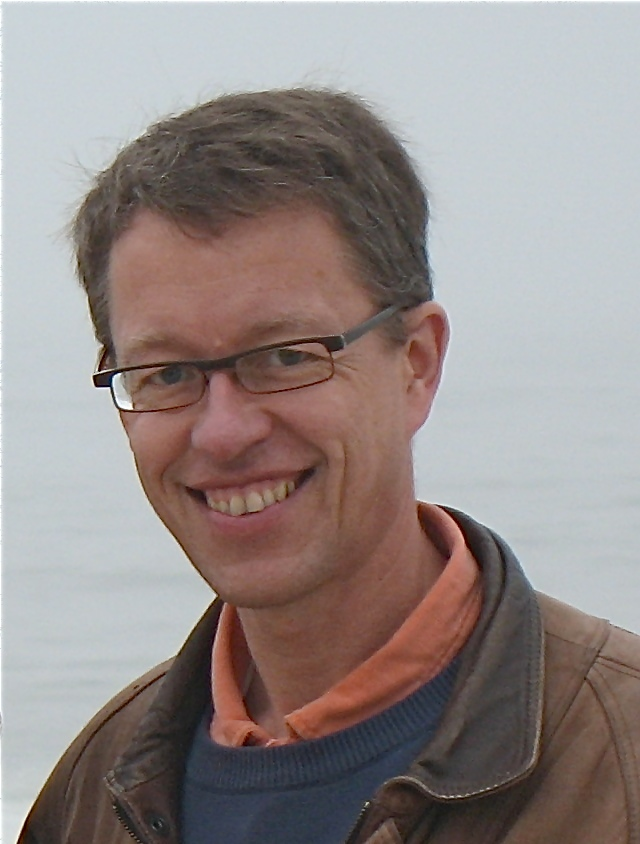
\includegraphics[height=1.5cm]{figs/Olivier.jpg}
%     & 
\includegraphics[height=1.5cm]{figs/Morgan.jpg} \\
%       \tval{Olivier ROUX} & \tval{Morgan MAGNIN} \\
%       Professeur \& chef d'équipe & Maître de conférences
%   \end{tabular}}\right\}$ %\text{\tval{MeForBio}}$%}
%   \parbox{2cm}{\tval{MeForBio}\\IRCCyN\\(Nantes, France)}
% 
%   \vspace*{3em}
%   $\left.\text{\begin{tabular}{c}
%     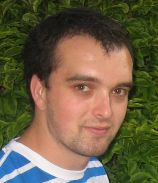
\includegraphics[height=1.5cm]{figs/Loic.jpg} \\ \tval{Loïc PAULEVÉ} \\ Chargé de recherche CNRS
%   \end{tabular}}\right\}$%\text{\tval{AMIB}}$
%   \parbox{1.5cm}{\tval{Bioinfo/AMIB}\\LRI\\(Orsay, France)}
%   \hspace*{3em}
%   $\left.\text{\begin{tabular}{c}
%     
\includegraphics[height=1.5cm]{figs/Inoue-sensei.jpg} \\ \tval{Katsumi INOUE} \\ Professeur \& chef d'équipe
%   \end{tabular}}\right\}$%\text{\tval{Inoue Laboratory}}$
%   \parbox{1.5cm}{\tval{Inoue Lab.}\\NII\\(Tokyo, Japon)}
% \end{center}

\end{frame}



\begin{frame}[c]
  \frametitle{Contributions personnelles}

\small
\emphcolor{Chapitre de livre :}
\begin{itemize}
  \item Paulevé, Chancellor, \tval{Folschette}, Magnin, Roux :\\
    \tval{Analyzing Large Network Dynamics with Process Hitting},\\
    \textit{Logical Modeling of Biological Systems},
%    éditeurs : Luis Farinas del Cerro et Katsumi Inoue,
    août 2014%, ISBN 978-1-84821-680-8.
\end{itemize}

\medskip
\emphcolor{Conférences et workshops :}
\begin{itemize}
  \item \tval{Folschette}, Paulevé, Magnin, Roux :\\
    \tval{Under-approximation of reachability in multivalued asynchronous networks},\\
    CS2Bio'13,
    %in: Proceedings of the fourth International Workshop on Interactions between Computer Science and Biology,
    %éditeurs : Emanuela Merelli et Angelo Troina,
    \textit{Electronic Notes in Theoretical Computer Science}, \vol 299, 2013\\
    \emphcolor{sélectionné pour un numéro spécial} de \textit{Theoretical Computer Science}
    %33--51, Springer Berlin Heidelberg, juin 2013, DOI 10.1016/j.entcs.2013.11.004.
    %\emphcolor{Selected for a special issue in the journal \textit{Theoretical Computer Science}.}
  \item \tval{Folschette}, Paulevé, Inoue, Magnin, Roux :\\
    \tval{Concretizing the process hitting into biological regulatory networks},\\ %\newline{}
    CMSB'12, \textit{Lecture Notes in Computer Science}, %éditeurs : David Gilbert et Monika Heiner, %\newline{}
    2012
    %in: \textit{Computational Methods in Systems Biology}, éditeurs : David Gilbert et Monika Heiner, %\newline{}
    %166--186, Springer Berlin Heidelberg, octobre 2012, DOI 10.1007/978-3-642-33636-2\_11.
  \item \tval{Folschette}, Paulevé, Inoue, Magnin, Roux :\\
    \tval{Abducing Biological Regulatory Networks from Process Hitting models},\\
    \textit{ECML-PKDD'12 / LDSSB'12}, %éditeurs : Oliver Ray et Katsumi Inoue,
    2012
    %24--35, septembre 2012.
\end{itemize}

\emphcolor{Soumissions de journaux en cours :}
\begin{itemize}
  \item \tval{Folschette}, Paulevé, Magnin, Roux :\\
    \tval{Sufficient Conditions for Reachability in Automata Networks with Priorities},\\
    %version étendue de “Under-approximation of reachability in multivalued asynchronous networks”,
    \emphcolor{soumis} à un numéro spécial de \textit{Theoretical Computer Science}% en avril 2014.
  \item \tval{Folschette}, Paulevé, Inoue, Magnin, Roux :\\
    \tval{Constructing Biological Regulatory Networks from Process Hitting models},\\
    %extended version of “Concretizing the process hitting into biological regulatory networks”,
    \emphcolor{en cours de révision} pour \textit{Theoretical Computer Science}
  \item Paulevé, \tval{Folschette}, Magnin, Roux :\\
    \tval{Analyses statiques de la dynamique des réseaux d'automates indéterministes},\\
    \emphcolor{soumis} à un numéro spécial de \textit{Technique et Science Informatiques}
    %editors: N.~Fatès and S.~Sené,
    %\emphcolor{soumis} en avril 2014.
\end{itemize}

\end{frame}


% 
% \begin{frame}[c]
%   \frametitle{Contributions personnelles}
% 
% \small
% \emphcolor{Chapitre de livre} avec Paulevé, Chancellor, Magnin, Roux :
% \begin{itemize}
%   \item \tval{Analyzing Large Network Dynamics with Process Hitting},\\
%     \textit{Logical Modeling of Biological Systems},
% %    éditeurs : Luis Farinas del Cerro et Katsumi Inoue,
%     2014%, ISBN 978-1-84821-680-8.
% \end{itemize}
% 
% \medskip
% \emphcolor{Workshop} avec Paulevé, Magnin, Roux :
% \begin{itemize}
%   \item \tval{Under-approximation of reachability in multivalued asynchronous networks},\\
%     CS2Bio'13,
%     %in: Proceedings of the fourth International Workshop on Interactions between Computer Science and Biology,
%     %éditeurs : Emanuela Merelli et Angelo Troina,
%     \textit{Electronic Notes in Theoretical Computer Science}, \vol 299, 2013\\
%     \emphcolor{sélectionné pour un numéro spécial} de \textit{Theoretical Computer Science}
%     %33--51, Springer Berlin Heidelberg, juin 2013, DOI 10.1016/j.entcs.2013.11.004.
%     %\emphcolor{Selected for a special issue in the journal \textit{Theoretical Computer Science}.}
% \end{itemize}
% 
% \emphcolor{Conférence et workshop} avec Paulevé, Inoue, Magnin, Roux :
% \begin{itemize}
%   \item \tval{Concretizing the process hitting into biological regulatory networks},\\ %\newline{}
%     CMSB'12, \textit{Lecture Notes in Computer Science}, %éditeurs : David Gilbert et Monika Heiner, %\newline{}
%     2012
%     %in: \textit{Computational Methods in Systems Biology}, éditeurs : David Gilbert et Monika Heiner, %\newline{}
%     %166--186, Springer Berlin Heidelberg, octobre 2012, DOI 10.1007/978-3-642-33636-2\_11.
%   \item \tval{Abducing Biological Regulatory Networks from Process Hitting models},\\
%     \textit{ECML-PKDD'12 / LDSSB'12}, %éditeurs : Oliver Ray et Katsumi Inoue,
%     2012
%     %24--35, septembre 2012.
% \end{itemize}
% 
% \emphcolor{Soumissions de journaux en cours :}
% \begin{itemize}
%   \item \tval{Folschette}, Paulevé, Magnin, Roux :\\
%     \tval{Sufficient Conditions for Reachability in Automata Networks with Priorities},\\
%     %version étendue de “Under-approximation of reachability in multivalued asynchronous networks”,
%     \emphcolor{soumis} à un numéro spécial de  de \textit{Theoretical Computer Science}% en avril 2014.
%   \item \tval{Folschette}, Paulevé, Inoue, Magnin, Roux :\\
%     \tval{Constructing Biological Regulatory Networks from Process Hitting models},\\
%     %extended version of “Concretizing the process hitting into biological regulatory networks”,
%     \emphcolor{en cours de révision} pour \textit{Theoretical Computer Science}
%   \item Paulevé, \tval{Folschette}, Magnin, Roux :\\
%     \tval{Analyses statiques de la dynamique des réseaux d'automates indéterministes},\\
%     \emphcolor{soumis} à un numéro spécial de \textit{Technique et Science Informatiques}
%     %editors: N.~Fatès and S.~Sené,
%     %\emphcolor{soumis} en avril 2014.
% \end{itemize}
% 
% \end{frame}
